% !TEX encoding = UTF-8 Unicode

\documentclass[aspectratio=169]{beamer}
\usepackage[utf8]{inputenc}

%% BIB
\usepackage[
  style=authoryear,
  backend=biber,
  url=false,
  maxcitenames=2,
  uniquename=false,
  uniquelist=false
]{biblatex}
%\addbibresource{?.bib}

%% GRAPHICS

\usepackage{graphicx}
\graphicspath{{images/},{figures/}}
\usepackage{tikz}

%% COLORS
\definecolor{UWRed}{HTML}{C5050C}
\definecolor{TintedBG}{HTML}{EEEEFF}
%\definecolor{StrongBlue}{HTML}{3F8FD2}
%\definecolor{StrongGreen}{HTML}{36C88E}
%\definecolor{StrongRed}{HTML}{9B0000}
%\definecolor{MyC}{HTML}{009999}
%\definecolor{MyM}{HTML}{990099}
%\definecolor{MyY}{HTML}{999900}
%\definecolor{MyR}{HTML}{990000}
%\definecolor{MyG}{HTML}{009900}
%\definecolor{MyB}{HTML}{000099}
%\definecolor{ActionRed}{HTML}{990000}

%% SLIDE COLOR SETTINGS
\setbeamercolor{structure}{fg=UWRed}
\setbeamercolor{title page}{fg=white}
\setbeamercolor{title}{fg=white}

%% RM NAV SYMBOLS
\setbeamertemplate{navigation symbols}{}

%% FONTS
\setbeamerfont{title}{size=\huge\bfseries}

%% DRAWING
%\usetikzlibrary{}

%% LOGO on slides
%\logo{\begin{tikzpicture}[overlay]
%  \node[anchor=north east,inner sep=0] at (0,86mm) {
\includegraphics[height=10mm]{SMPH_color-flush.pdf}};
%\end{tikzpicture}}

%% CONTENT BEGINS

\title{Craven Group Meeting}
\author{Yuriy Sverchkov}
\institute{University of Wisconsin--Madison}
\date{February 7, 2020}

\begin{document}
	
	\begin{frame}[plain]
		\raggedleft
		
\includegraphics[width=\linewidth]{lakkaraju-2019-title.png} \\
		\vfill
		\it Presentation by Yuriy Sverchkov \\
		\textbf{Craven Group Meeting} \\ February 7, 2020
	\end{frame}


	\begin{frame}{The need for model explanation}
		
		\begin{itemize}
			\item Many of the best-performing machine learning models are not (easily) \textbf{interpretable} (by non-ML experts) \pause
			\item Users need explanations:
			\begin{itemize}
				\item when using models for medical decisions
				\item when using models for policymaking
				\item in other high-risk decision support
				\item for legal reasons
			\end{itemize}
		\end{itemize}
		\pause
		
		\textbf{GDPR Article 13(2f)} [The data subject shall be informed of] the existence of automated decision-making [... and provided] meaningful information about the logic involved
		\pause
		
		\begin{itemize}
			\item Explanations build trust in a good model
			\item Explanations can help troubleshoot a bad model
		\end{itemize}
	\end{frame}
	
	
	\begin{frame}{Interpretable models}
		\begin{columns}
			\column[T]{0.45\textwidth}
			\begin{center}\bf Interpretable \end{center} \pause
			\begin{itemize}
				\item Generalized linear models
				\item[] $y = g^{-1}( X\beta )$ \pause
				\item[] For each feature $i$, $\beta_i$ tells us about its contribution:
				\begin{itemize}
					\item sign (e.g. increase vs. decrease of a risk due to a factor)
					\item magnitude (relative importance of features)
				\end{itemize} \pause
				\item Rules and decision trees
				%\item [] example?
			\end{itemize} \pause
			
			\column[T]{0.45\textwidth}
			\begin{center}\textbf{Uninterpretable} or "black box"\end{center}
			\centering
			\only<5-6>{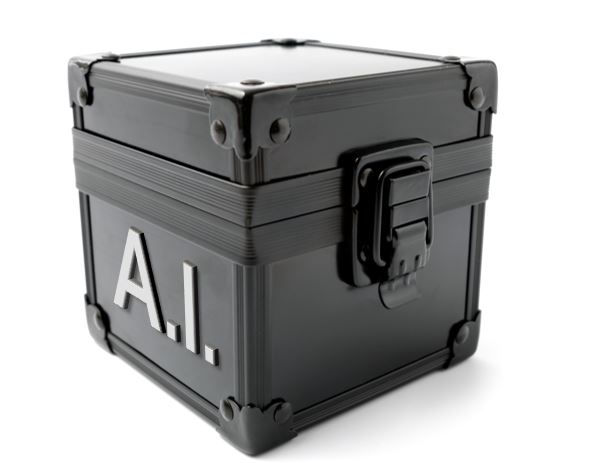
\includegraphics[height=2.5cm]{AI-Box.jpg}} \pause
			\only<7->{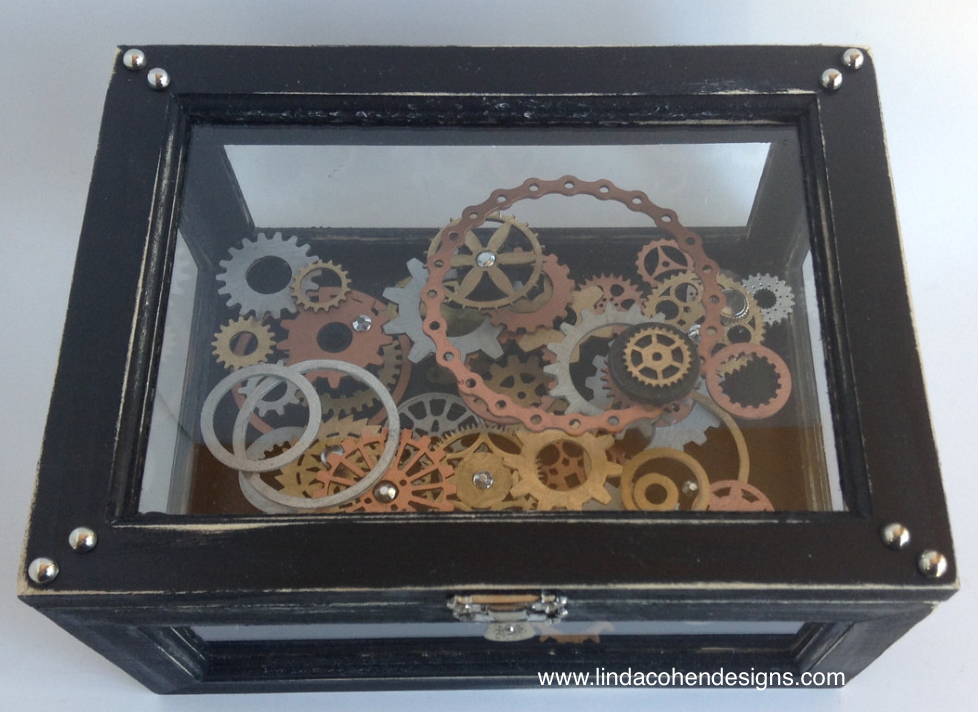
\includegraphics[height=2.5cm]{glass-gear-box.png}}
			\begin{itemize}
				\item e.g. 3-layer neural network
				\item[] $y = \sigma( W^1 \sigma( W^2 \sigma( W^3 X ) ) )$
				\item[] \textbf{what does a particular value of $W^2_{ij}$ mean? \pause }
				\item We can look in the box, but it's hard to interpret.
			\end{itemize}
			
		\end{columns}
		\vfill
		\scriptsize
		Image credit: \url{fico.com} ; \url{www.lindacohendesigns.com}
	\end{frame}

	% Problem statement
	
	\begin{frame}{Lakkaraju, Kamar, Caruana and Leskovec 2019}
		\centering
		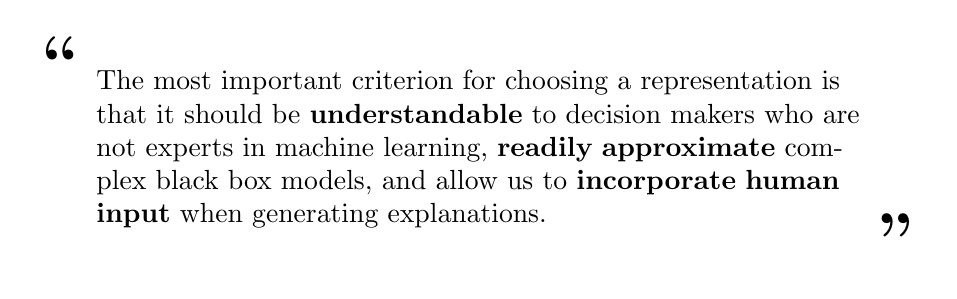
\begin{tikzpicture}
			\node (q) {\bf\textrm{\Huge``}};
			\node (t) [anchor=north west, text width=0.8\linewidth, align=left] at (q.east)
				{The most important criterion for choosing a representation is that it
				should be \textbf{understandable} to decision makers who are not experts in
				machine learning, \textbf{readily approximate} complex black box models,
				and allow us to \textbf{incorporate human input} when generating explanations.};
			\node [anchor=west] at (t.south east) {\bf\textrm{\Huge''}};
		\end{tikzpicture}		
	\end{frame}

	\begin{frame}{Representation}
		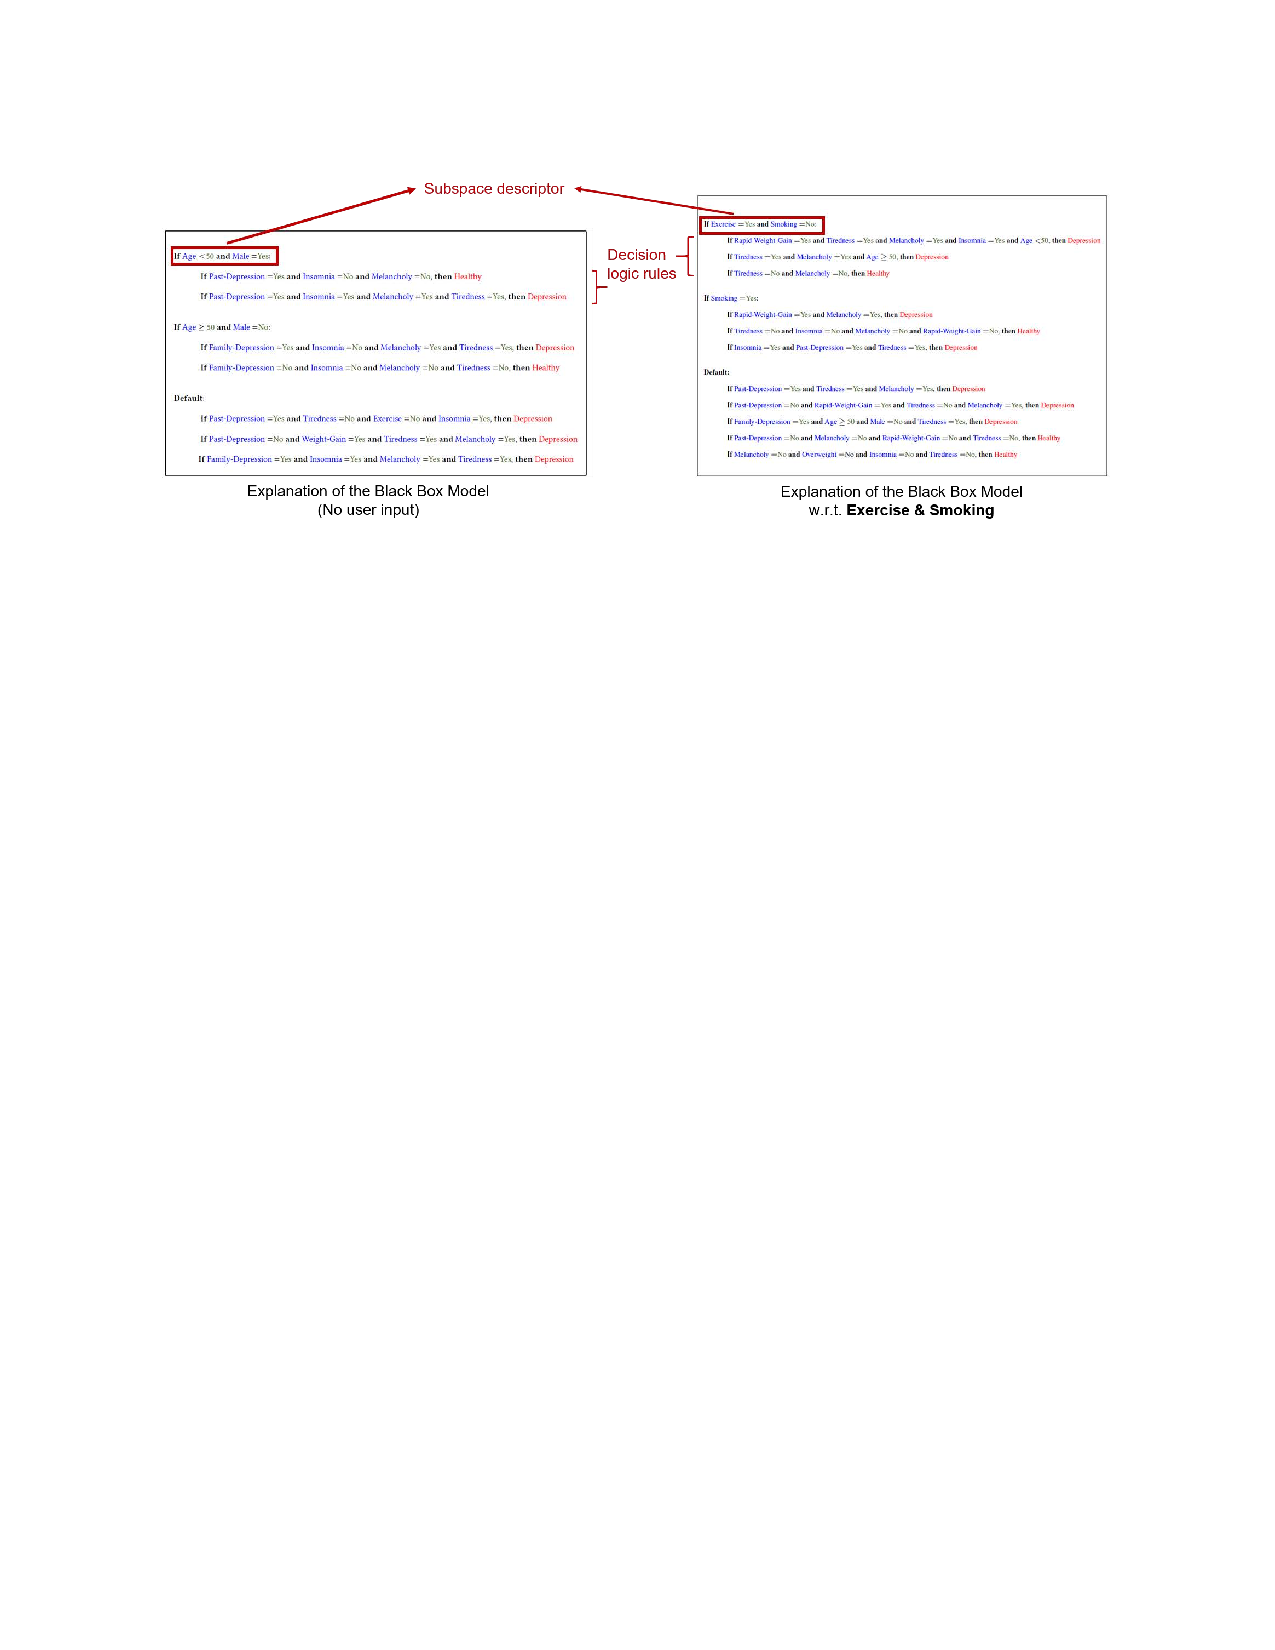
\includegraphics[width=\linewidth]{lakkaraju-fig-1}
	\end{frame}

	\begin{frame}
		\centering
		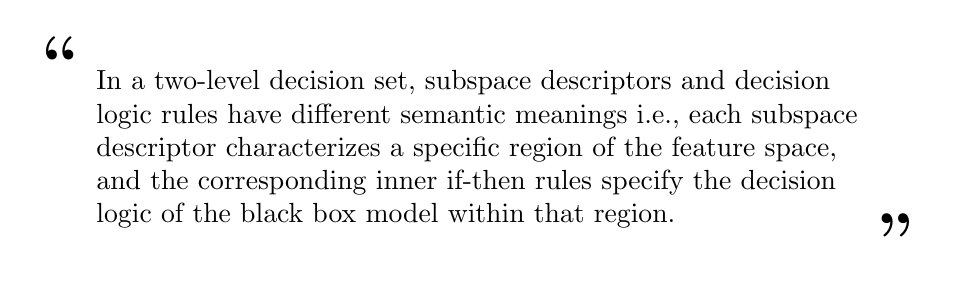
\begin{tikzpicture}
		\node (q) {\bf\textrm{\Huge``}};
		\node (t) [anchor=north west, text width=0.8\linewidth, align=left] at (q.east)
		{In a two-level decision set, subspace descriptors and decision
			logic rules have different semantic meanings i.e., each subspace
			descriptor characterizes a specific region of the feature space, and
			the corresponding inner if-then rules specify the decision logic of
			the black box model within that region.};
		\node [anchor=west] at (t.south east) {\bf\textrm{\Huge''}};
		\end{tikzpicture}
	\end{frame}

	\begin{frame}
		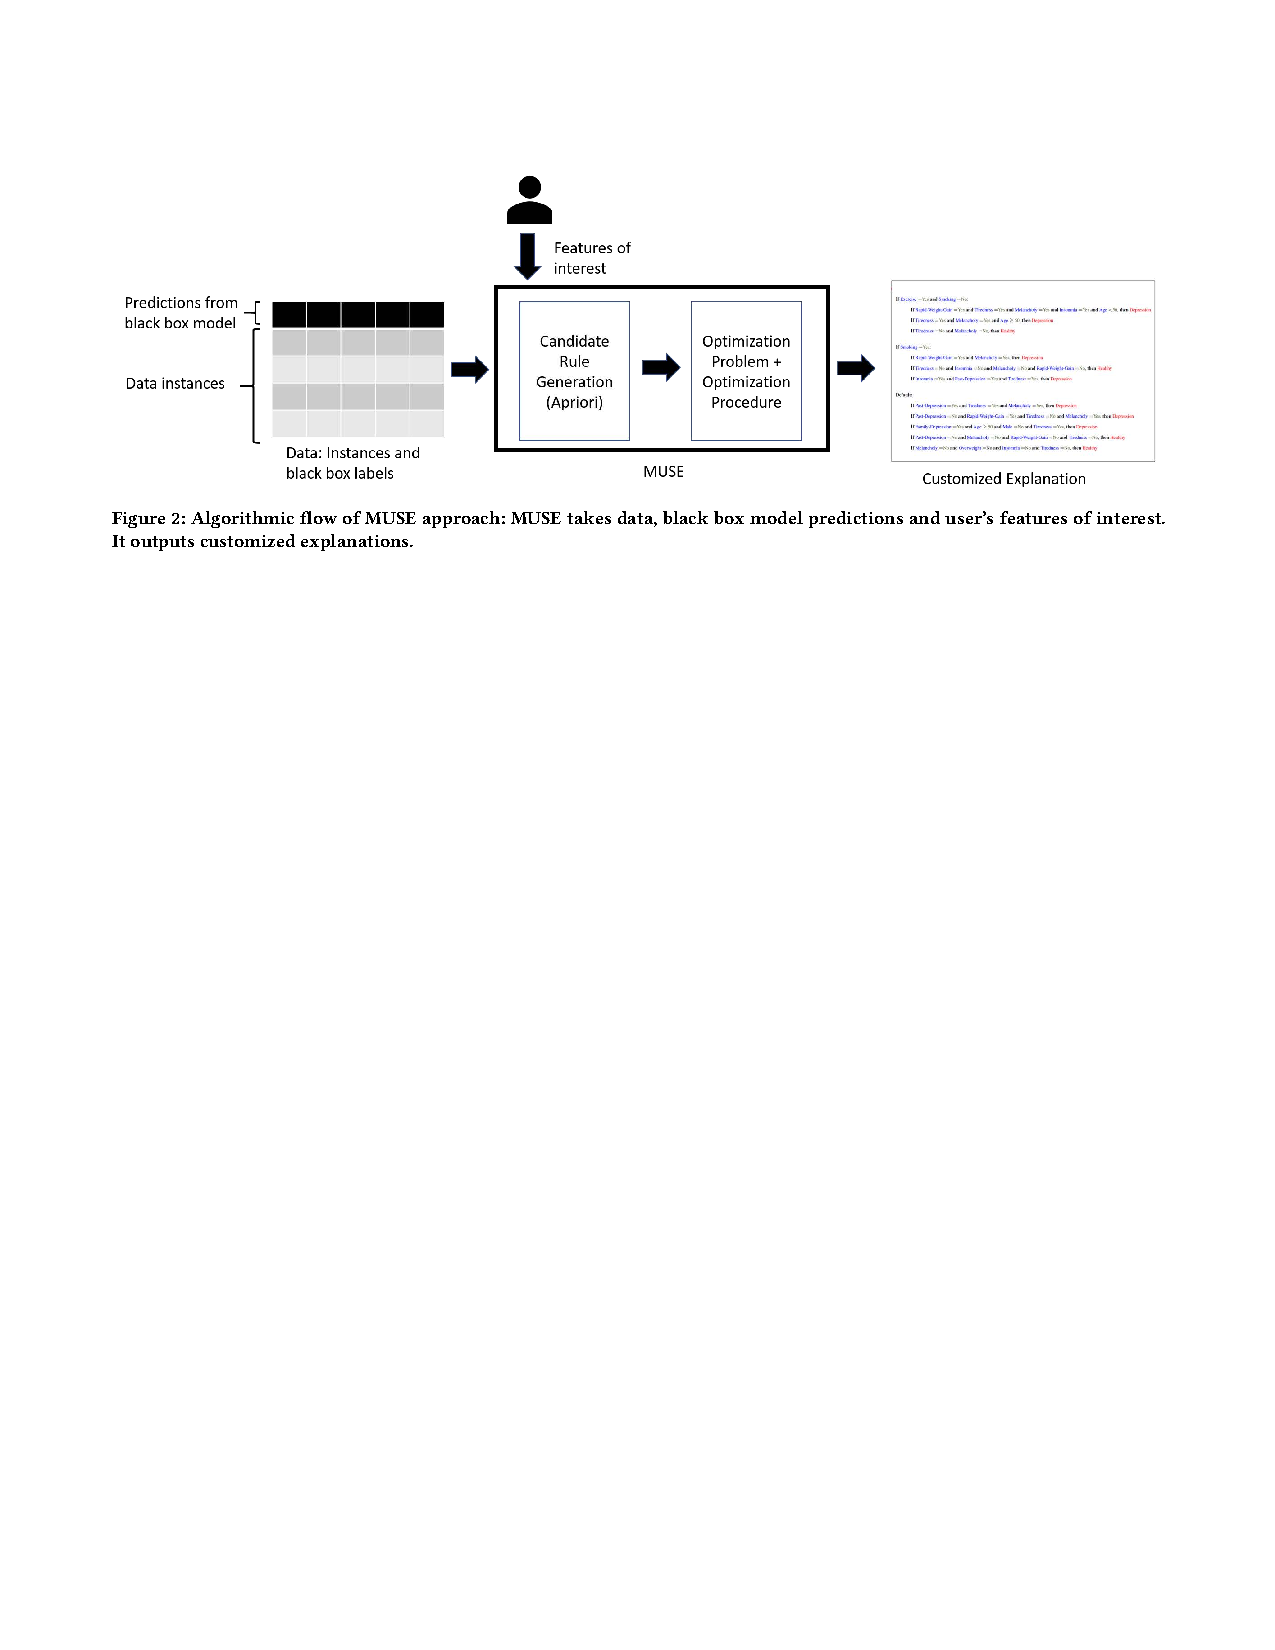
\includegraphics[width=\linewidth]{lakkaraju-fig-2}
	\end{frame}

	\begin{frame}{Agrawal and Srikant, VLDB 1994}
		\begin{columns}
			\column{0.6\linewidth}
			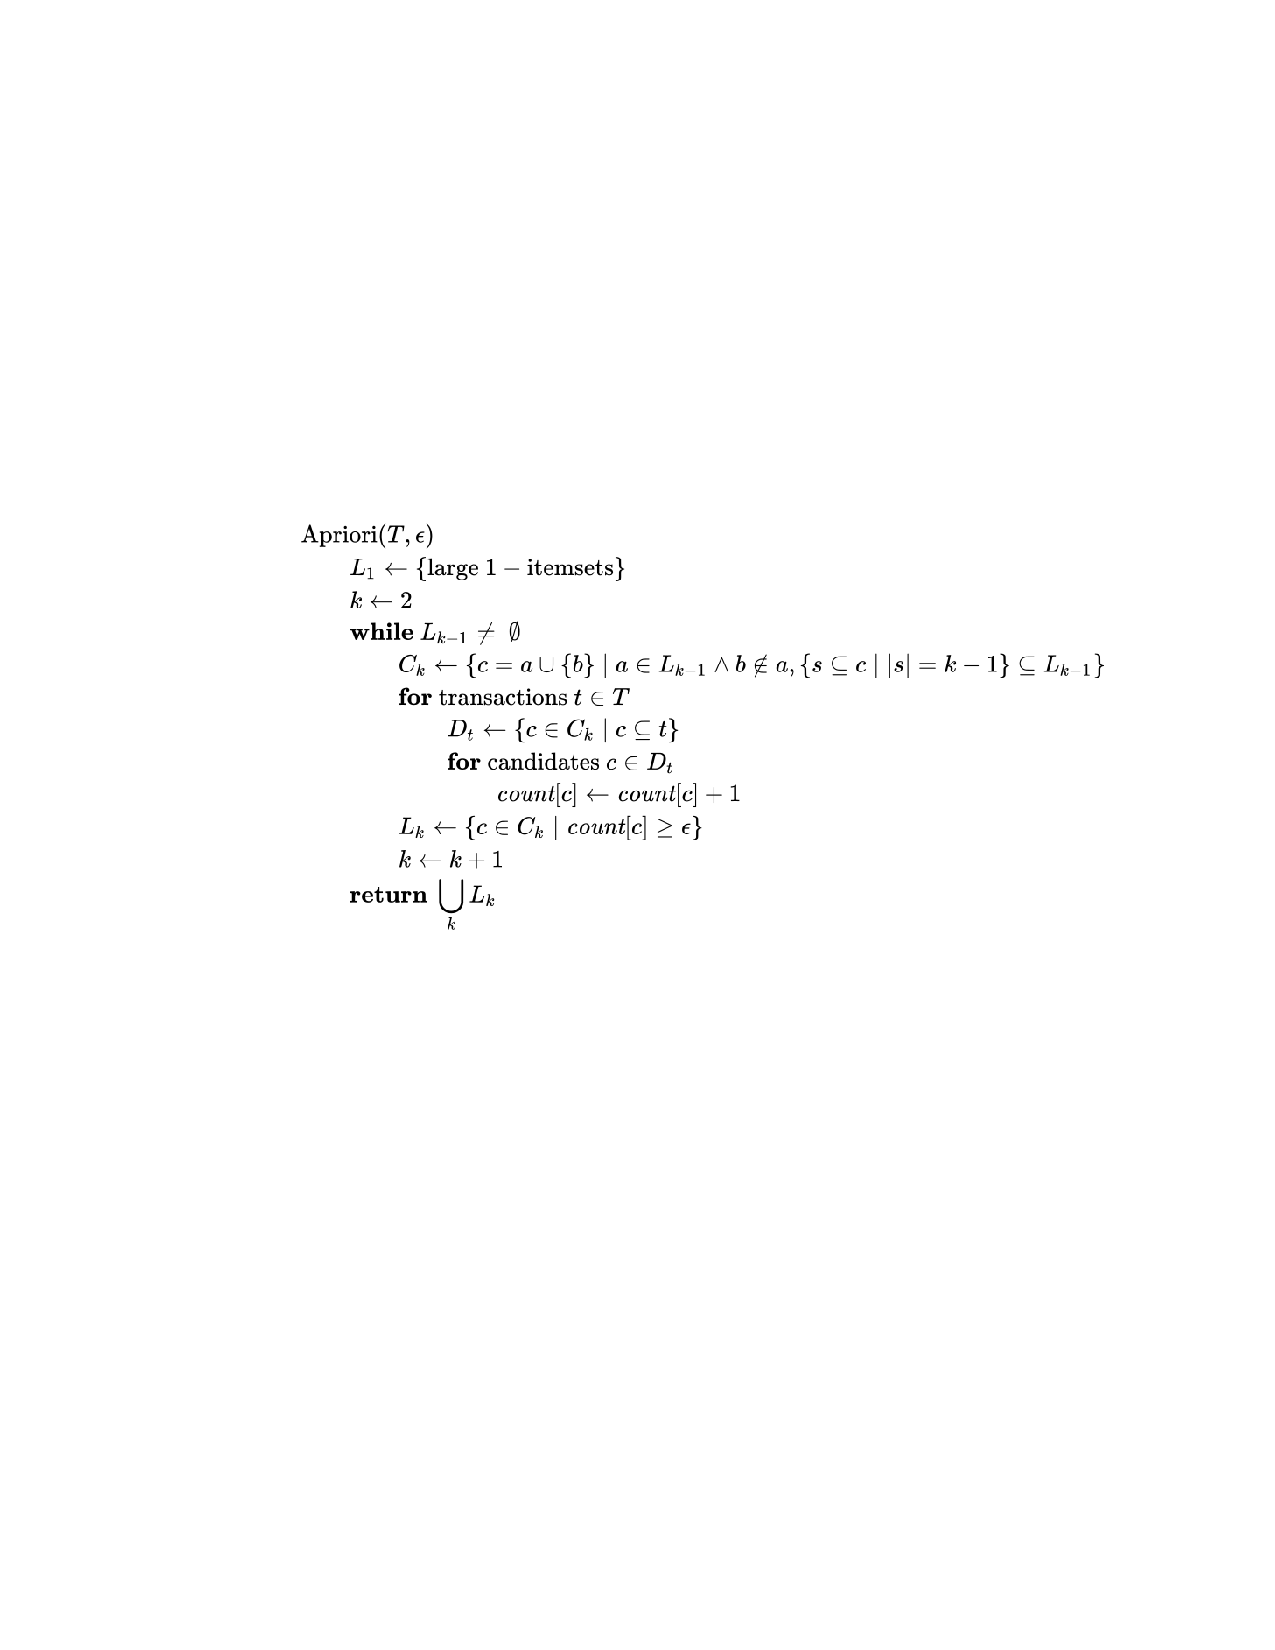
\includegraphics[width=\linewidth]{apriori-alg}
			\column{0.37\linewidth}
			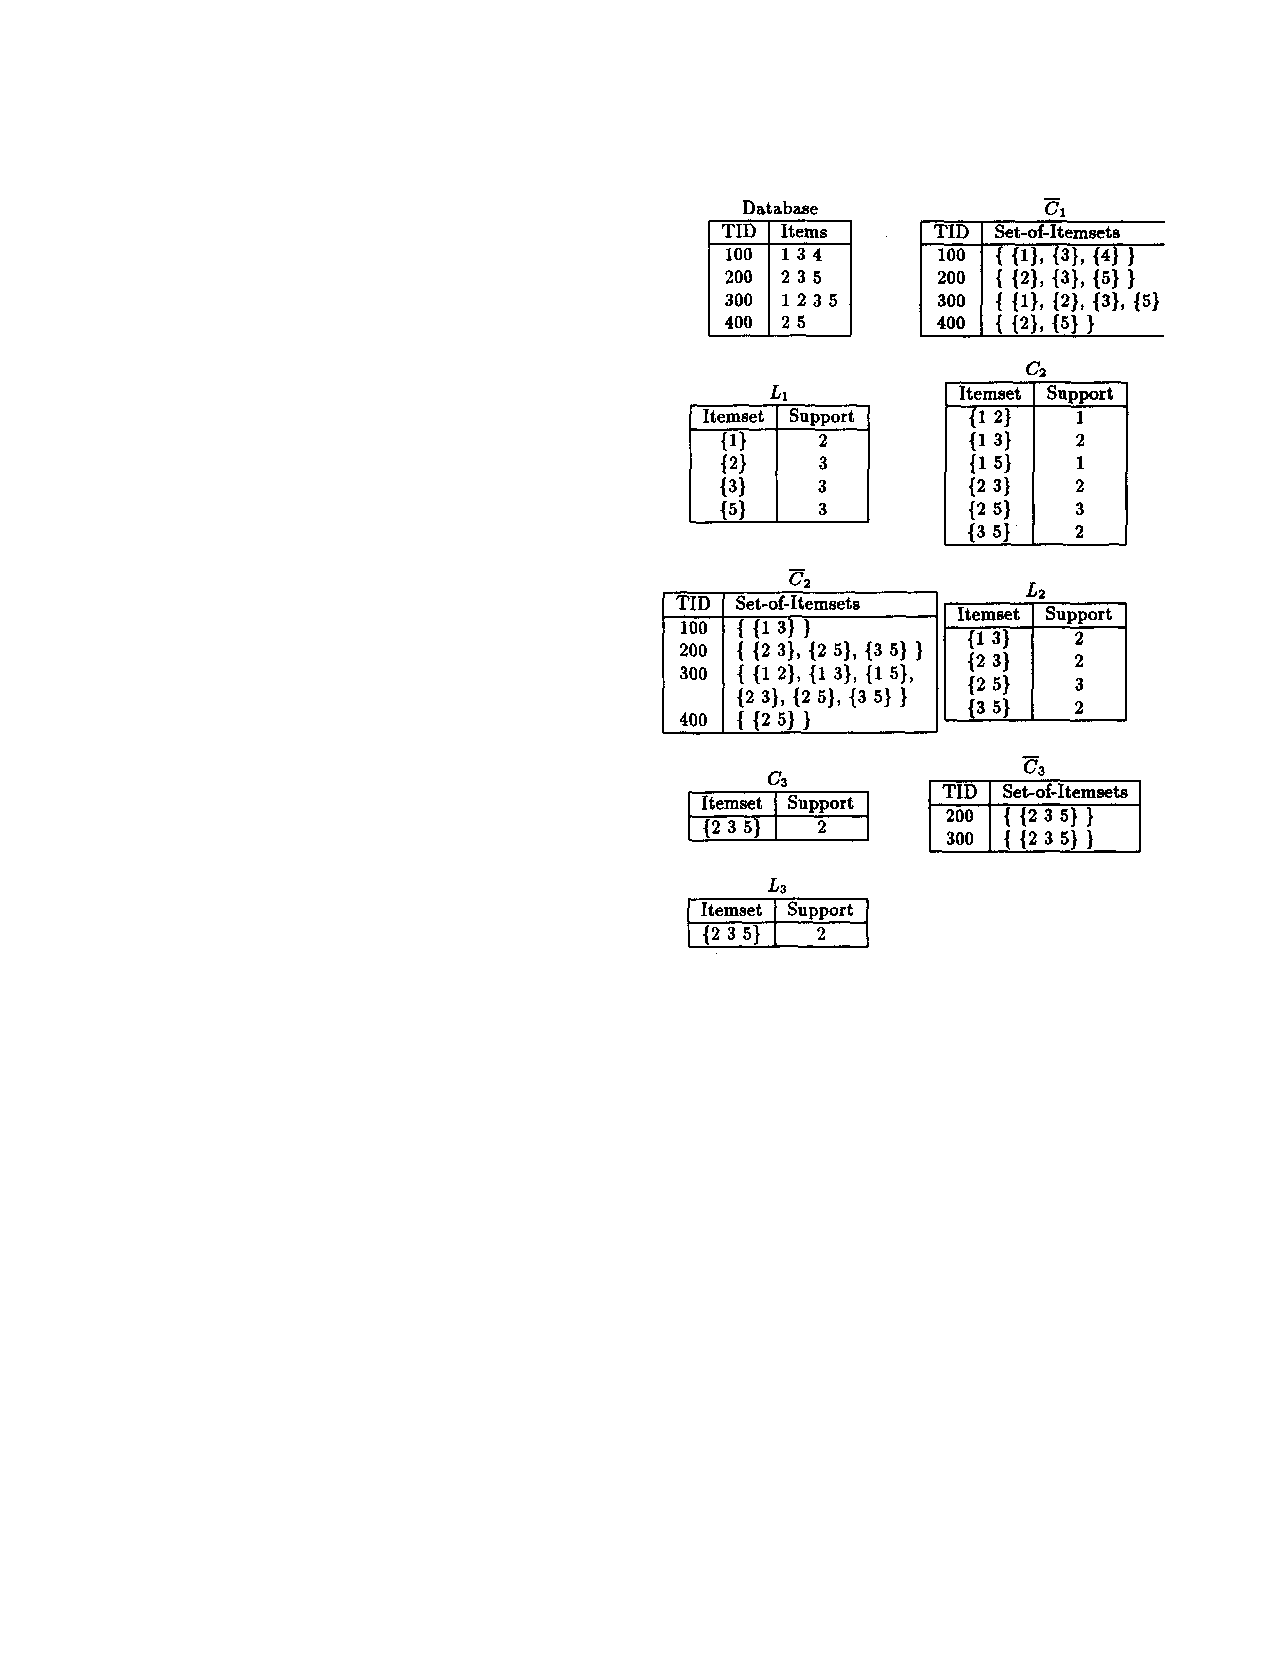
\includegraphics[width=\linewidth]{apriori-ex}
		\end{columns}
	\end{frame}

	%\begin{frame}{Representation}
	%	
	%	Two level decision set
	%	
	%	$\{ (q_i, s_i, c_i) | i \in 1, \ldots, M \}$
	%	
	%	where $q_i$ and $s_i$ are conjunctions (`and') of 1-feature predicates
	%	($q_i$ - `subspace descriptors'; $s_i$ - `decision logic rules')
	%	
	%	where $c_i$ are class labels
	%	
	%	There's a tie-breaking function if multiple sets apply to an instance (they chose rule that has higher agreement with black box) % TODO check how exactly that's defined
	%	
	%	There's a default class if no sets apply to an instance (they chose the majority class according to the black box) % TODO is this a majority given some set of instances
	%	
	%\end{frame}

	% Note: we are defining measures w.r.t. a two-level decision set \mathcal R with M rules,
	% a black box \mathcal B, and a dataset \mathcal D = \{ \mathbf x_i | i \in 1, \ldots, N\}
	%
	% Fidelity: disagreement( \mathcal R ) = number of instances (in \mathcal D?) where
	% \mathcal R and \mathcal B do not yield the same class c
	%
	% Unambiguity:
	% ruleoverlap( \mathcal R ) : number of rules above 1 that explain an instance (instances?)
	% cover( \mathcal R ) : coverage of the instance space by rules
	% Unambiguity is achieved by max cover and min ruleoverlap
	%
	% Interpretability:
	% size( \mathcal R ) = M
	% maxwidth( \mathcal R ) = max\{ width(s_i), width(q_i) | (q_i, s_i, c_i) \in \mathcal R \}
	% width( * ) is the number of predicates in *
	% numpreds( \mathcal R ) = total number of predicates
	% numdsets( \mathcal R ) = number of unique subspace descriptors
	% featureoverlap( \mathcal R ) = sum featureoverlap(q, s) 

	\begin{frame}
		
		\centering
		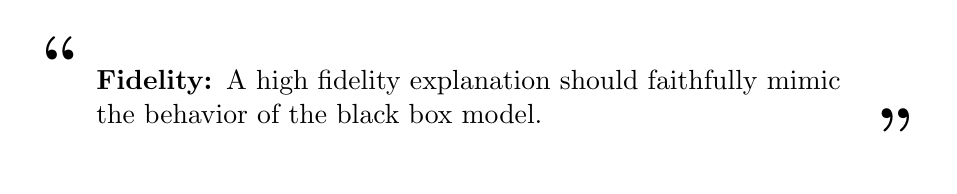
\begin{tikzpicture}
		\node (q) {\bf\textrm{\Huge``}};
		\node (t) [anchor=north west, text width=0.8\linewidth, align=left] at (q.east)
		{\textbf{Fidelity:} A high fidelity explanation should faithfully mimic the
			behavior of the black box model.};
		\node [anchor=west] at (t.south east) {\bf\textrm{\Huge''}};
		\end{tikzpicture}
		
		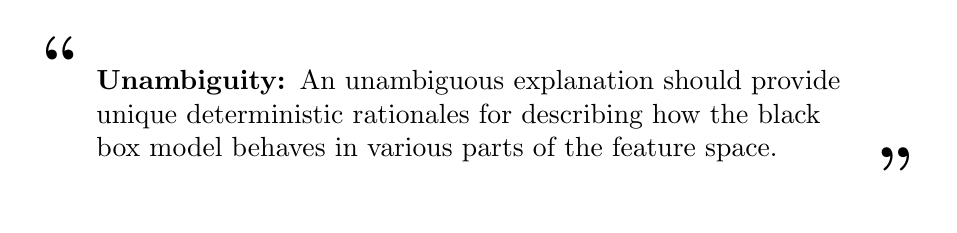
\begin{tikzpicture}
		\node (q) {\bf\textrm{\Huge``}};
		\node (t) [anchor=north west, text width=0.8\linewidth, align=left] at (q.east)
		{\textbf{Unambiguity:} An unambiguous explanation should provide
			unique deterministic rationales for describing how the black box
			model behaves in various parts of the feature space.};
		\node [anchor=west] at (t.south east) {\bf\textrm{\Huge''}};
		\end{tikzpicture}
		
		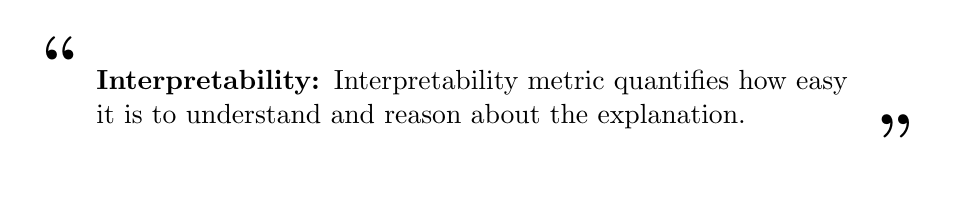
\begin{tikzpicture}
		\node (q) {\bf\textrm{\Huge``}};
		\node (t) [anchor=north west, text width=0.8\linewidth, align=left] at (q.east)
		{\textbf{Interpretability:} Interpretability metric quantifies how easy it
			is to understand and reason about the explanation.};
		\node [anchor=west] at (t.south east) {\bf\textrm{\Huge''}};
		\end{tikzpicture}

	\end{frame}

	\begin{frame}{Optimization problem}
		\begin{columns}
			\column{0.47\linewidth}
			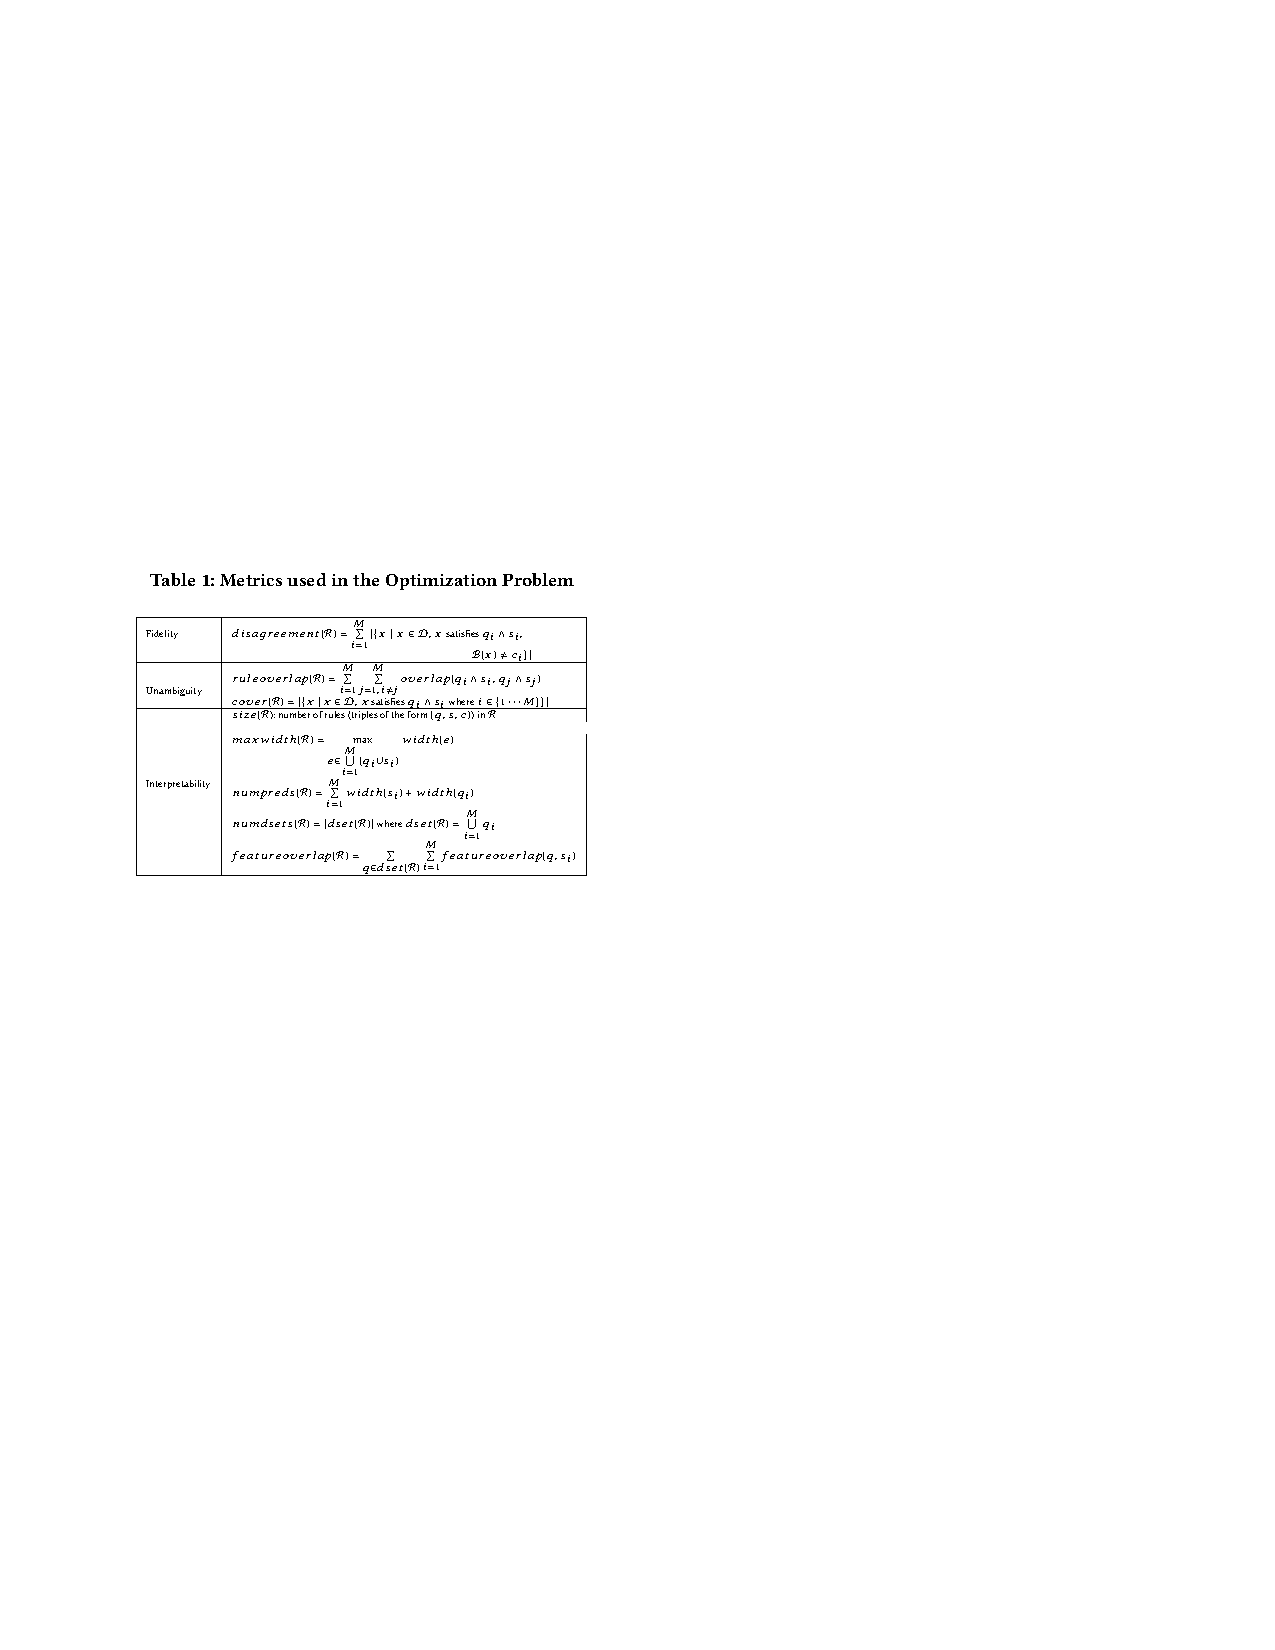
\includegraphics[width=\linewidth]{lakkaraju-table-1}
			\column{0.47\linewidth}
			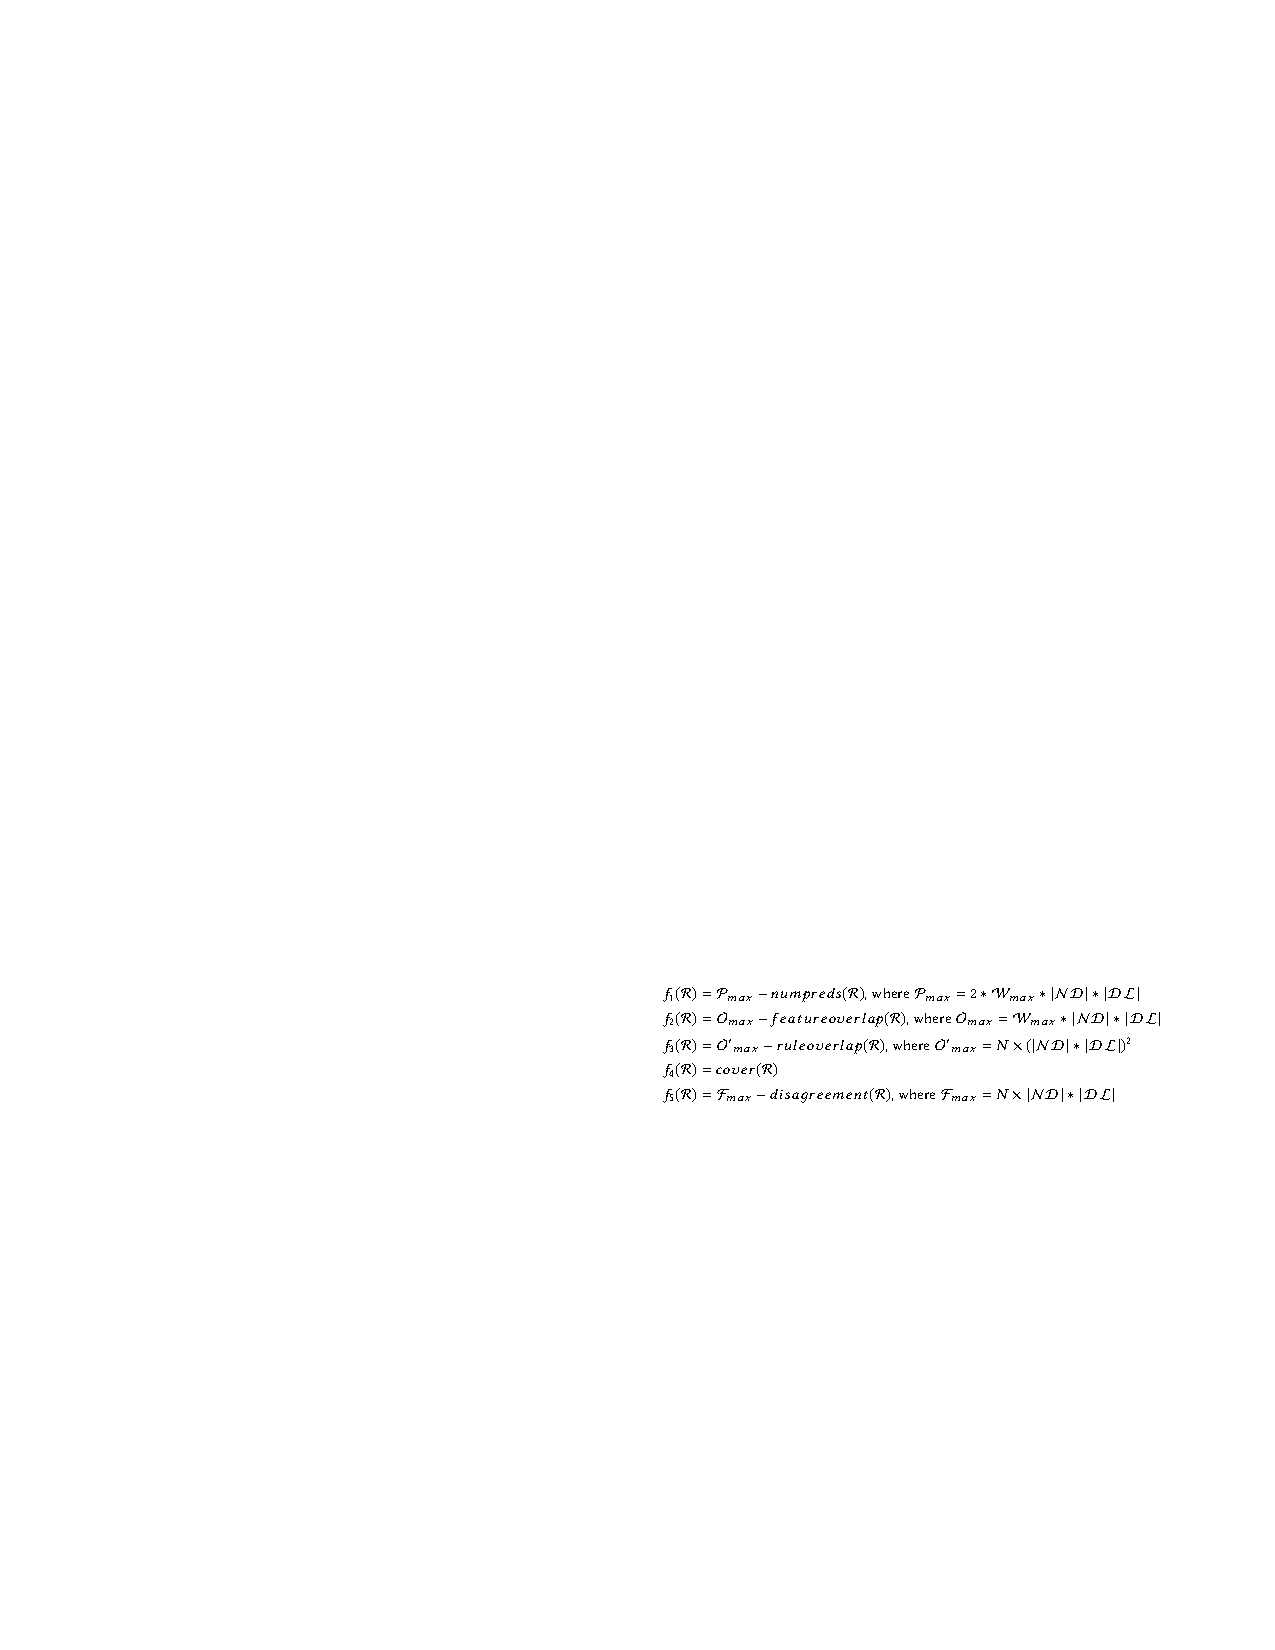
\includegraphics[width=\linewidth]{lakkaraju-objf} \\ \vspace{1cm}
			
\includegraphics[width=\linewidth]{lakkaraju-objf2}
		\end{columns}
	\end{frame}
	
	\begin{frame}
		\begin{itemize}
			\item They prove that the optimization problem
			\begin{itemize}
				\item is non-normal
				\item is non-negative
				\item is non-monotone
				\item is submodular
				\item has matroid constraints
			\end{itemize}
			\item The optimization procedure is based on approximate local search, which has optimality guarantees for this type of problem.
		\end{itemize}
	\end{frame}

	\begin{frame}
		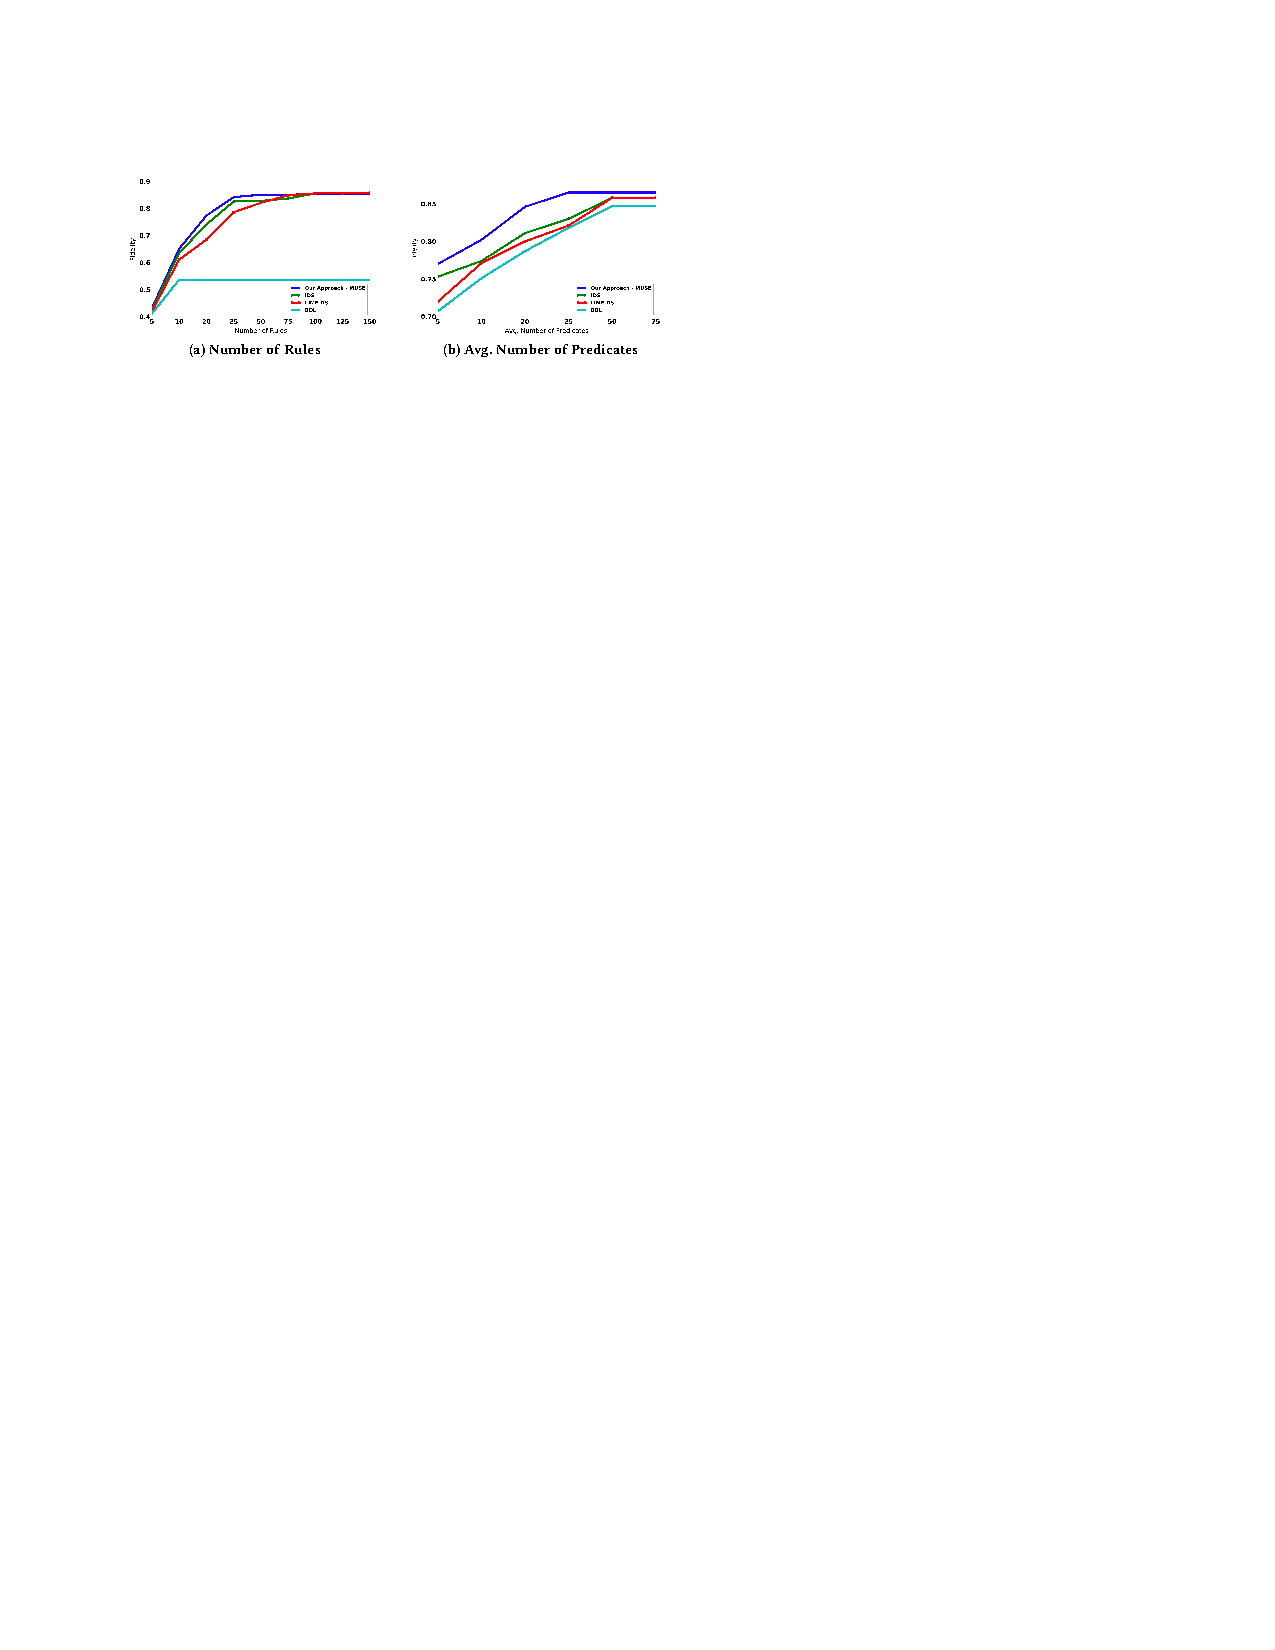
\includegraphics[width=\linewidth]{lakkaraju-fig-3ab}
	\end{frame}

	\begin{frame}{User study}
		\begin{columns}
			\column{0.5\linewidth}
			\begin{itemize}
				\item Participants were asked questions after seeing a model explanation.
				\item Given a case, what is the prediction?
				\item Given a case, what would need to hold true to result in a given prediction?
				\item ``Customized explanation'' customized w.r.t question by the investigators.
			\end{itemize}
			\column{0.45\linewidth}
			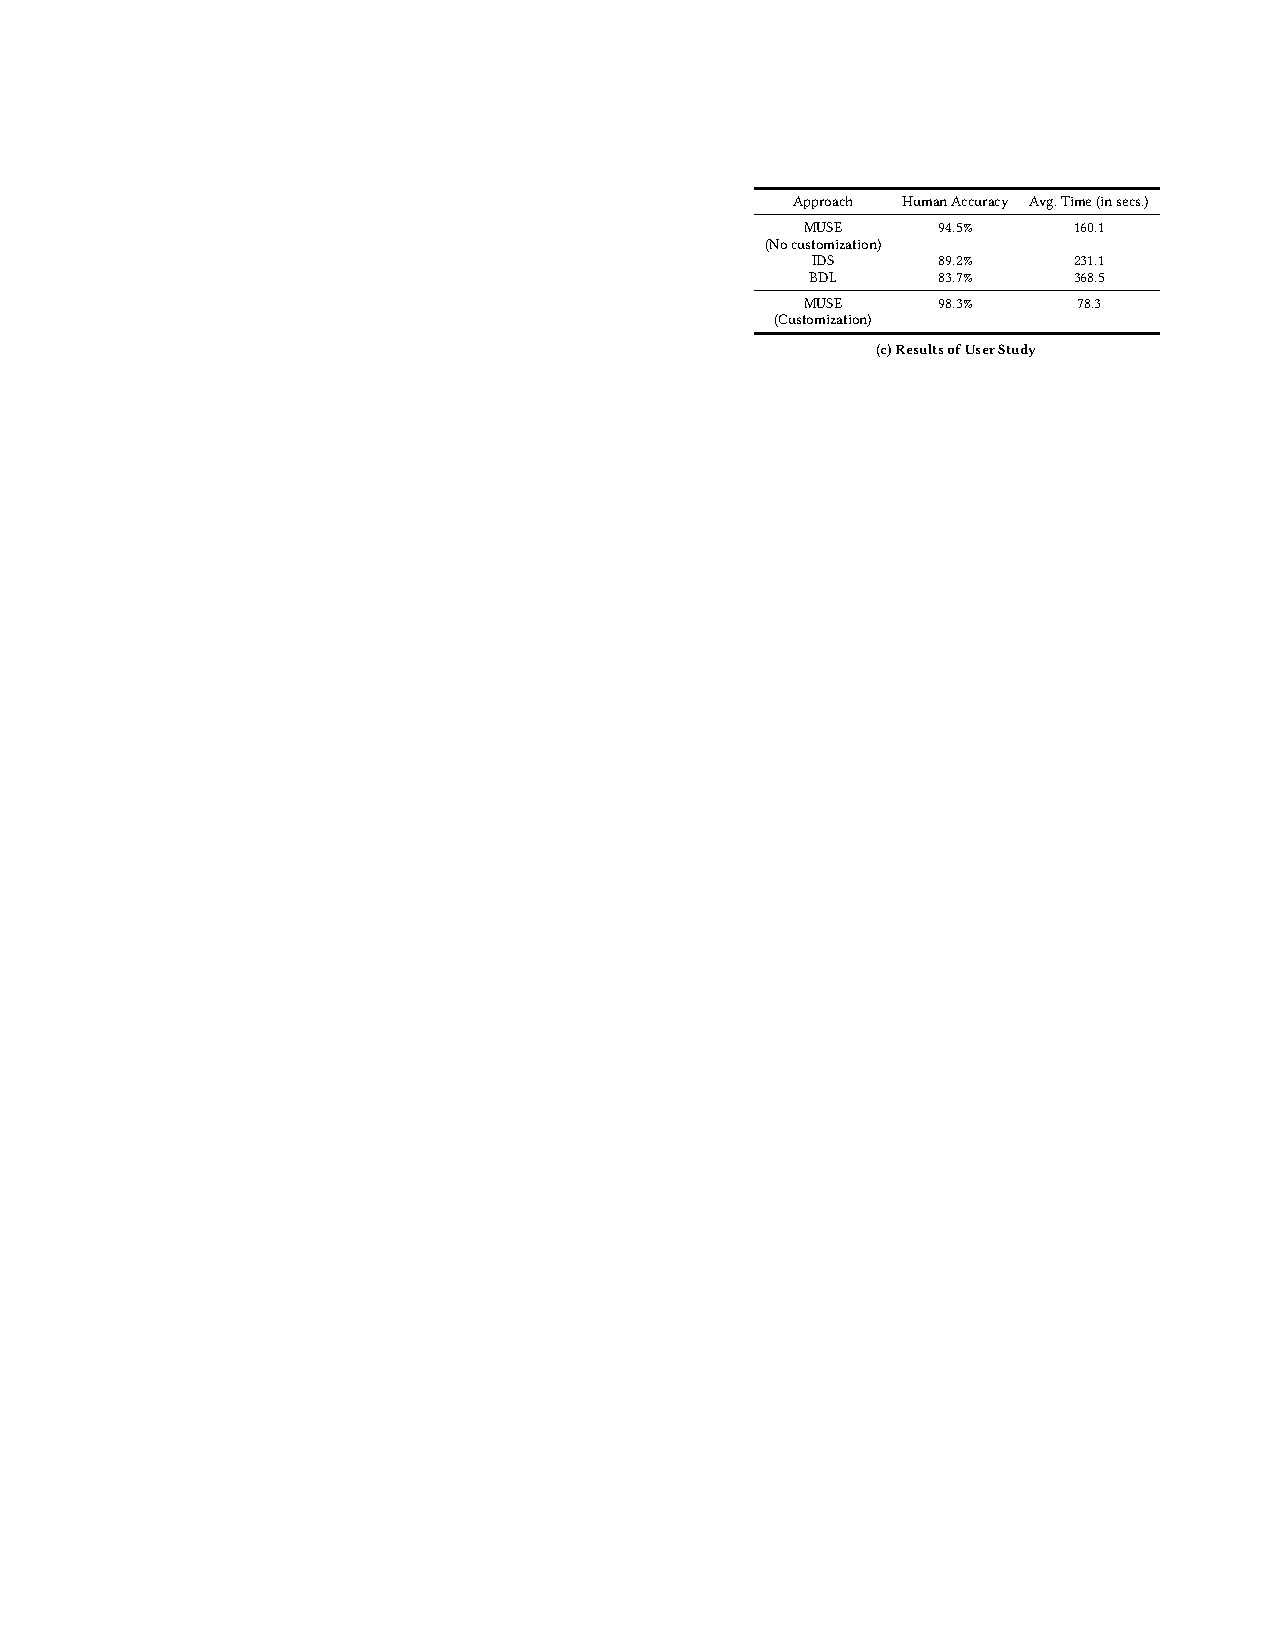
\includegraphics[width=\linewidth]{lakkaraju-fig-3c}
		\end{columns}
		
	\end{frame}


\begin{frame}{LIME}
\begin{columns}
	\column{0.47\textwidth} \centering
	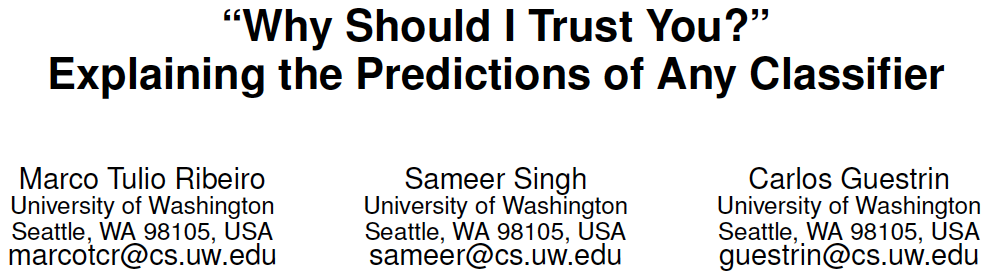
\includegraphics[width=6cm]{LIME-title.png}
	
	{\color{UWRed}
	\[
	\arg \min_g \underbrace{ \mathcal L ( f, g, \pi_x ) }_{\text{fidelity loss around }x} + \underbrace{ \Omega( g ) }_\text{complexity}
	\]}
	
	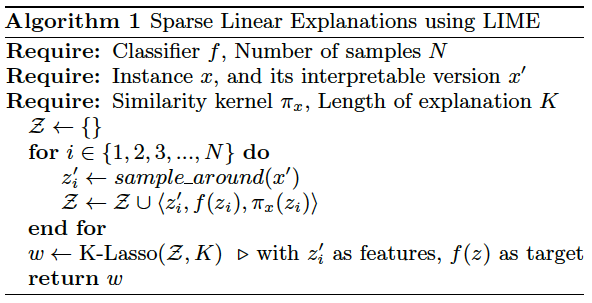
\includegraphics[width=6cm]{LIME-alg.png}
	\column{0.47\textwidth} \centering
	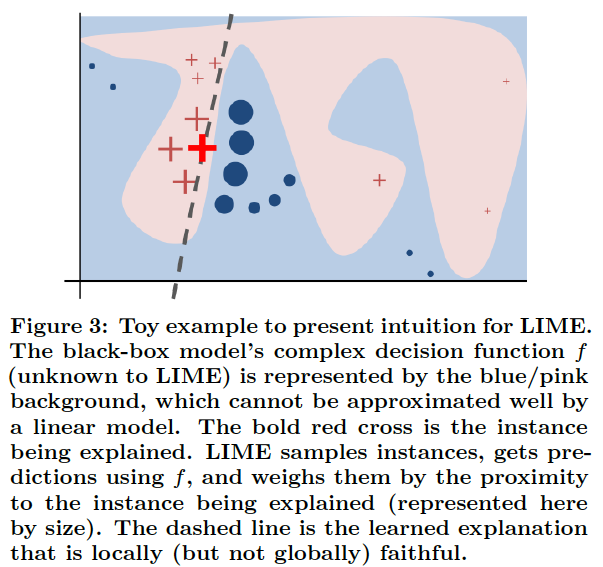
\includegraphics[width=6cm]{LIME-intuition.png}
\end{columns}
\end{frame}


\begin{frame}{LIME applied to images}
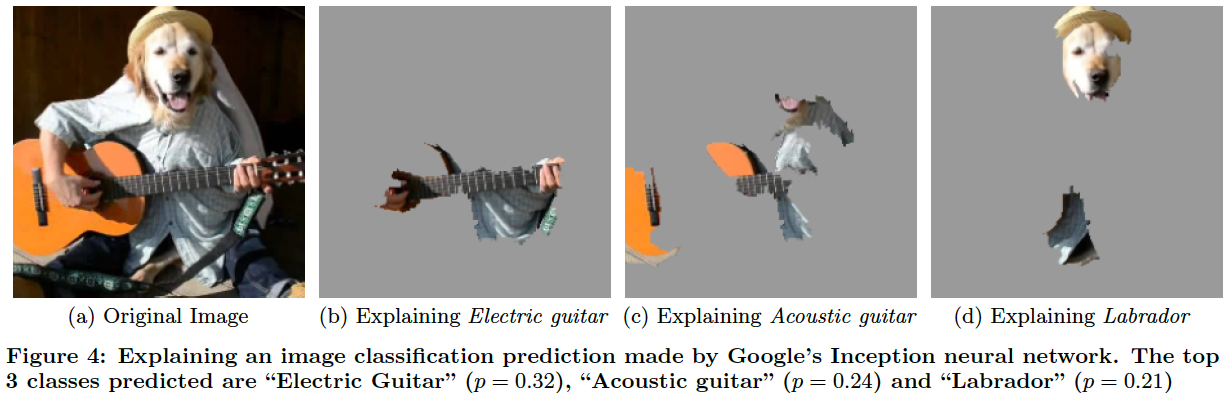
\includegraphics[width=\textwidth]{LIME-image.png}
\end{frame}

\end{document}